% hav plot for $r=\sqrt n$ med til forsvar

\documentclass{llncs}
\usepackage[utf8]{inputenc}
\usepackage{verbatim}
\usepackage{graphicx}
\usepackage{algorithm}
\usepackage{clrscode}
\usepackage[draft]{fixme}
\usepackage{amsmath}
%\usepackage{amsthm}
\usepackage{textcomp}
\usepackage{enumerate}

\usepackage{prettyref}
\newcommand{\sectionname}{Section}
% \renewcommand{\figurename}{Figure}
\newcommand*{\pref}{\prettyref}
% Adds varioref to the prettyrefs.
% Replacing vref with ref to avoid page numbers
\newrefformat{cha}{\chaptername~\ref{#1}}
\newrefformat{sec}{\sectionname~\ref{#1}}
\newrefformat{fig}{\figurename~\ref{#1}}
\newrefformat{eq}{\equationname~\ref{#1}}
\newrefformat{tab}{\tablename~\ref{#1}}
\newrefformat{app}{\appendixname~\ref{#1}}
\newrefformat{alg}{Algorithm~\ref{#1}}

\title{Longest Common Extensions via Fingerprinting} 

\author{Philip Bille \and Inge Li G{\o}rtz \and Jesper Kristensen}

\institute{Technical University of Denmark, DTU Informatics} 

%\date{}

%\newtheorem{theorem}{Theorem}
%\newtheorem{lemma}{Lemma}
%\newtheorem{corollary}{Corollary}

% http://texblog.net/latex/layout/page/2/
\fontdimen2\font=0.25em% interword space
\fontdimen3\font=1em% interword stretch
\fontdimen4\font=0.10em% interword shrink

\begin{document}

\maketitle

\newcommand{\sortt}{\textit{sort}(n,\sigma)}
\newcommand{\LCE}{\textit{LCE}}
\newcommand{\NCA}{\textit{NCA}}
\newcommand{\RMQ}{\textit{RMQ}}
\newcommand{\SA}{\textit{SA}}
\newcommand{\SAinv}{\textit{SA}^{-1}} % math
\newcommand{\SAi}{SA$^{-1}$} % no math
\newcommand{\LCP}{\textit{LCP}}
\newcommand{\LA}{\textit{LA}}
\newcommand{\suff}{\textit{suff}}
\newcommand{\logceil}{\lceil\log n\rceil}
\newcommand{\fprint}[1][k]{\ensuremath{\proc{Fingerprint}_{#1}}}
\newcommand{\fprintk}{\fprint[k]}
\newcommand{\RMQpq}[2]{RMQ\textless$#1$, $#2$\textgreater}
\newcommand{\RMQn}{\RMQpq{1}{n}}
\newcommand{\RMQq}{\RMQpq{n}{1}}
\newcommand{\RMQlog}{\RMQpq{n}{\log n}}

\hyphenation{Di-rect-Comp Di-rect-Look-up Di-rect-Comp-Look-up Fin-ger-print}

%\tableofcontents

%\vspace{1cm}
% stuff on toc page

%\newpage

\begin{abstract}
The \emph{longest common extension} (LCE) problem is to preprocess a string in order to allow for a large number of LCE queries, such that the queries are efficient. The LCE value, $\LCE_s(i,j)$, is the length of the longest common prefix of the pair of suffixes starting at index $i$ and $j$ in the string $s$. The LCE problem can be solved in linear space with constant query time and a preprocessing of sorting complexity. There are two known approaches achieving these bounds, which use nearest common ancestors and range minimum queries, respectively. However, in practice a much simpler approach with linear query time, no extra space and no preprocessing achieves significantly better average case performance. We show a new algorithm, \fprintk, which for a parameter $k$, $1\leq k\leq\logceil$, on a string of length $n$ and alphabet size $\sigma$, gives $O(k n^{1/k})$ query time using $O(k n)$ space and $O(k n + \sortt)$ preprocessing time, where $\sortt$ is the time it takes to sort $n$ numbers from $\sigma$. Though this solution is asymptotically strictly worse than the asymptotically best previously known algorithms, it outperforms them in practice in average case and is almost as fast as the simple linear time algorithm. On worst case input, this new algorithm is significantly faster in practice compared to the simple linear time algorithm. We also look at cache performance of the new algorithm, and we show that for $k=2$, cache optimization can improve practical query time.
\end{abstract}

%%%%%%%%%%%%%%%%%%%%%%%%%%%%%%%%%%%%%%%%%%%%%%%%%%%%%%%%%%%%%%%%%%%%%%%%%%%%%%%
%%%%%%%%%%%%%%%%%%%%%%%%%%%%%%%%%%%%%%%%%%%%%%%%%%%%%%%%%%%%%%%%%%%%%%%%%%%%%%%
\section{Introduction\label{sec:intro}}

The \emph{longest common extension} (LCE) problem is to preprocess a string in order to allow for a large number of LCE queries, such that the queries are efficient. The LCE value, $\LCE_s(i,j)$, is the length of the longest common prefix of the pair of suffixes starting at index $i$ and $j$ in the string $s$. The LCE problem can be used in many algorithms for solving other algorithmic problems, e.g., the Landau-Vishkin algorithm for approximate string searching~\cite{approx-search}. Solutions with linear space, constant query time, and $O(\sortt)$ preprocessing time exists for the problem~\cite{nca,jf-rmq}. Here $\sortt$ is the time it takes to sort $n$ numbers from an alphabet of size $\sigma$. For $\sigma=O(n^c)$, where $c$ is a constant, we have $\sortt=O(n)$. These theoretically good solutions are however not the best in practice, since they have large constant factors for both query time and space usage. Ilie et~al.~\cite{ilie-navarro-tinta} introduced a much simpler solution with average case constant time and no space or preprocessing required other than storing the input string. This solution has significantly better practical performance for average case input as well as for average case queries on some real world strings, when compared to the asymptotically best known algorithms. However, this algorithm has linear worst case query time, and is thus only ideal when worst case performance is irrelevant. In situations where we need both average case and worst case performance to be good, none of the existing solutions are ideal. Such a situation could be use of approximate string searching in a firewall. The firewall should not allow an attacker to significantly degrade its performance by sending it carefully crafted packages. At the same time it must scan legitimate data fast. The main goal of this paper is to design an algorithm that performs well in both situations, that is, achieves a good worst-case guarantee while maintaining a fast average case performance.

% PB: har slettet nedenst�ende afsnit til fordel for ekstra s�tning i ovenst�ende. Resultaterne kommer senere.
%In this paper we give a new algorithm, which is a generalization of the simple linear time algorithm. The new algorithm is almost as simple, yet it has significantly better worst case query time. This algorithm also achieves significantly better average case practical query time compared to the asymptotically best known worst case query time algorithms. The algorithm uses string fingerprinting inspired by Karp-Miller-Rosenberg~\cite{karp-miller-rosenberg} to achieve a time/space-tradeoff with $O(k n^{1/k})$ worst case query time, constant average case query time, and $O(kn)$ space for any integer $k$, $1 \leq k \leq \log n$, on a string of length $n$. The preprocessing time for this algorithm is $O(kn+\sortt)$. We look at a cache optimization for the new fingerprinting based algorithm, which improves query I/O for small values of $k$, and we show that for $k=2$, this cache optimization improves practical query times.

%%%%%%%%%%%%%%%%%%%%%%%%%%%%%%%%%%%%%%%%%%%%%%%%%%%%%%%%%%%%%%%%%%%%%%%%%%%%%%%
%\subsection{Previous Results\label{sec:existing-results}}
\paragraph{Previous Results\label{sec:existing-results}}
Thoughout the paper let $s$ be a string of length $n$ over alphabet of size $\sigma$. Ilie~et~al.~\cite{ilie-navarro-tinta} gave an algorithm, \proc{DirectComp}, for solving the LCE problem, which uses no preprocessing and has $O(\LCE(i,j))$ query time. For a query $\LCE(i,j)$, the algorithm simply compares $s[i]$ to $s[j]$, then $s[i+1]$ to $s[j+1]$ and so on, until the two characters differ, or the end of the string is reached. The worst case query time is thus $O(n)$. However, on random strings and many real-word texts Ilie~et~al.~\cite{ilie-navarro-tinta} showed that the average LCE is $O(1)$, where the average is over all $\sigma^n n^2$ combinations of strings and query inputs. Hence, in these scenarios \proc{DirectComp} achieves $O(1)$ query time. 

%Given a string length $n$ and an alphabet size $\sigma$, we define \emph{average case query time} as the average of query times over all $\sigma^n n^2$ combinations of strings and query inputs. 

The LCE problem can also be solved with $O(1)$ worst case query time, using $O(n)$ space and $O(\sortt)$ preprocessing time. Essentially, two different ways of doing this exists. One method, \proc{SuffixNca}, uses constant time nearest common ancestor (NCA) queries~\cite{nca} on a suffix tree. The LCE of two indexes $i$ and $j$ is defined as the length of the longest common prefix of the suffixes $s[i\twodots n]$ and $s[j\twodots n]$. In a suffix tree, the path from the root to $L_i$ has label $s[i\twodots n]$ (likewise for $j$), and no two child edge labels of the same node will have the same first character. The longest common prefix of the two suffixes will therefore be the path label from the root to the nearest common ancestor of $L_i$ and $L_j$, i.e., $\LCE_s(i,j) = D[\NCA_\mathcal{T}(L_i,L_j)]$.
The other method, \proc{LcpRmq}, uses constant time range minimum queries (RMQ)~\cite{jf-rmq} on a longest common prefix (LCP) array. The LCP array contains the length of the longest common prefixes of each pair of neighbor suffixes in the suffix array (SA). The length of the longest common prefix of two arbitrary suffixes in SA can be found as the minimum of all LCP values of neighbor suffixes between the two desired suffixes, because SA lists the suffixes in lexicographical ordering, i.e., $\LCE(i,j)=\LCP[\RMQ_{\LCP}(\SAinv[i] + 1, \SAinv[j])]$, where $\SAinv[i] < \SAinv[j]$. \pref{tab:article-algorithms} summaries the above theoretical bounds.
 
%Hence, it is interesting to have LCE algorithms, which perform good on average when the LCE value is small. Both \proc{SuffixNca} and \proc{LcpRmq} have the same asymptotic space and times. In practice, \proc{LcpRmq} is the best of the two~\cite{ilie-navarro-tinta}. The constant factor for average case query time of \proc{DirectComp} is much smaller than the constant factor for query time of \proc{LcpRmq}, thus \proc{DirectComp} is better in practice on average case inputs than the theoretically best \proc{LcpRmq}.

%%%%%%%%%%%%%%%%%%%%%%%%%%%%%%%%%%%%%%%%%%%%%%%%%%%%%%%%%%%%%%%%%%%%%%%%%%%%%%%
%\subsection{Our Results}
\paragraph{Our Results}
We present a new LCE algorithm, \fprintk, based on multiple levels of string fingerprinting. The algorithm has a parameter $k$ in the range $1\leq k\leq\logceil$, which describes the number of levels used\footnote{All logarithms are base two.}. The performance of the algorithm is summarized by the following theorem:
\begin{theorem}
For a string $s$ of length $n$ and alphabet size $\sigma$, the \fprintk\ algorithm, where $k$ is a parameter $1 \leq k \leq \logceil$, can solve the LCE problem in $O(k n^{1/k})$ worst case query time and $O(1)$ average case query time using $O(k n)$ space and $O(\sortt + k n)$ preprocessing time.
\end{theorem}
By choosing $k$ we can obtain the following interesting tradeoffs.
\begin{corollary}
\fprint[1] is equivalent to \proc{DirectComp} with $O(n)$ space and $O(n)$ query time.
\end{corollary}
\begin{corollary}
\fprint[2] uses $O(n)$ space and $O(\sqrt n)$ query time. It has two levels, where one uses a table of fingerprints and the other uses the original string.
\end{corollary}
\begin{corollary}
\fprint[\logceil] uses $O(n\log n)$ space and $O(\log n)$ query time. The data structure is equivalent to the one generated by Karp-Miller-Rosenberg~\cite{karp-miller-rosenberg}, and a query only needs to do one comparison at each level.
\end{corollary}
To preprocess the $O(k n)$ fingerprints used by our algorithm, we can use Karp-Miller-Rosenberg~\cite{karp-miller-rosenberg}, which takes $O(n\log n)$ time. For $k=o(\log n)$, we can speed up preprocessing to $O(\sortt + k n)$ by using the SA and LCP arrays.

\pref{tab:article-algorithms} shows an overview of asymptotic bounds of the different LCE algorithms.

\begin{table}[tb]
\centering
% \begin{tabular}{l|p{160px}|p{160px}}
\begin{tabular}{l|l|l|l}
\hline\hline
Algorithm & Space & Query time & Preprocessing \\ [0.5ex] \hline
\proc{SuffixNca} & $O(n)$ & $O(1)$ & $O(\sortt)$ \\ \hline
\proc{LcpRmq} & $O(n)$ & $O(1)$ & $O(\sortt)$ \\ \hline
\proc{DirectComp} & $O(1)$ & $O(n)$ & None \\ \hline
\fprintk * & $O(k n)$ & $O(k n^{1/k})$ & $O(\sortt+k n)$ \\
~~~~$k=\logceil$ * & $O(n\log n)$ & $O(\log n)$ & $O(n\log n)$ \\ \hline \\
\end{tabular}
\caption{LCE algorithms with their space requirements, worst case query times and preprocessing times. Average case query times are $O(1)$ for all shown algorithms. Rows marked with * show the new algorithm we present.}\label{tab:article-algorithms}
\end{table}

In practice, existing state of the art solutions are either good in worst case, while poor in average case (\proc{LcpRmq}), or good in average case while poor in worst case (\proc{DirectComp}). Our \fprintk\ solution targets a worst case vs. average case query time tradeoff between these two extremes. Our solution is almost as fast as \proc{DirectComp} on an average case input, and it is significantly faster than \proc{DirectComp} on a worst case input. Compared to \proc{LcpRmq}, our solution has a significantly better performance on an average case input, but its worst case performance is not as good as that of \proc{LcpRmq}. The space usage for \proc{LcpRmq} and \fprintk\ are approximately the same when $k=6$.

For $k=2$ we can improve practical \fprintk\ query time even further by optimizing it for cache efficiency. However for $k>2$, this cache optimization degrades practical query time performance, as the added overhead outweighs the improved cache efficiency.

Our algorithm is fairly simple. Though it is slightly more complicated than \proc{DirectComp}, it does not use any of the advanced algorithmic techniques required by \proc{LcpRmq} and \proc{SuffixNca}.

%%%%%%%%%%%%%%%%%%%%%%%%%%%%%%%%%%%%%%%%%%%%%%%%%%%%%%%%%%%%%%%%%%%%%%%%%%%%%%%
%\subsection{Overview}
%\paragraph{Overview}
%In \pref{sec:fprintk} we present the \fprintk\ algorithm and analyze its theoretical complexity, and in \pref{sec:results} we present our findings from tests of a practical implementation of \fprintk, which we compare against the existing algorithms.

%%%%%%%%%%%%%%%%%%%%%%%%%%%%%%%%%%%%%%%%%%%%%%%%%%%%%%%%%%%%%%%%%%%%%%%%%%%%%%%
%%%%%%%%%%%%%%%%%%%%%%%%%%%%%%%%%%%%%%%%%%%%%%%%%%%%%%%%%%%%%%%%%%%%%%%%%%%%%%%
\section{Preliminaries}

% \paragraph{String notation.}
Let $s$ be a string of length $n$. Then $s[i]$ is the $i$'th character of $s$, and $s[i\twodots j]$ is a substring of $s$ containing characters $s[i]$ to $s[j]$, both inclusive. That is, $s[1]$ is the first character of $s$, $s[n]$ is the last character, and $s[1\twodots n]$ is the entire string. The suffix of $s$ starting at index $i$ is written $\suff_i = s[i\twodots n]$.
%\paragraph{Sorting complexity.}
%The time it takes to sort $n$ numbers within an universe of size $\sigma$ is written as $\sortt$.

%\paragraph{Suffix tree.}
A \emph{suffix tree} $\mathcal{T}$ encodes all suffixes of a string $s$ of length $n$ with alphabet $\sigma$. The tree has $n$ leaves named $L_1$ to $L_n$, one for each suffix of $s$. Each edge is labeled with a substring of $s$, such that for any $1\leq i\leq n$, the concatenation of labels on edges on the path from the root to $L_i$ gives $\suff_i$. Any internal node must have more than one child, and the labels of two child edges must not share the same first character. The string depth $D[v]$ of a node $v$ is the length of the string formed when concatenating the edge labels on the path from the root to $v$.
The tree uses $O(n)$ space, and building it takes $O(\sortt)$ time~\cite{sort-complexity}.

%\paragraph{SA and LCP.}
For a string $s$ of length $n$ with alphabet size $\sigma$, the \emph{suffix array} (\SA) is an array of length $n$, which encodes the lexicographical ordering of all suffixes of $s$. The lexicographically smallest suffix is $\suff_{\SA[1]}$, the lexicographically largest suffix is $\suff_{\SA[n]}$, and the lexicographically $i$'th smallest suffix is $\suff_{\SA[i]}$. The \emph{inverse suffix array} (\SAi) describes where a given suffix is in the lexicographical order. Suffix $\suff_i$ is the lexicographically $\SAinv[i]$'th smallest suffix.

The \emph{longest common prefix array} (LCP array) describes the length of longest common prefixes of neighboring suffixes in SA. The length of the longest common prefix of $\suff_{\SA[i-1]}$ and $\suff_{\SA[i]}$ is $\LCP[i]$, for $2 \leq i \leq n$. The first element $\LCP[1]$ is always zero.
Building the SA, \SAi\ and LCP arrays takes $O(\sortt)$ time~\cite{sort-complexity}.

%\paragraph{NCA.}
The \emph{nearest common ancestor} (NCA) of two nodes $u$ and $v$ in a tree is the node of greatest depth, which is an ancestor of both $u$ and $v$. The ancestors of a node $u$ includes $u$ itself. An NCA query can be answered in $O(1)$ time with $O(n)$ space and preprocessing time in a static tree with $n$ nodes~\cite{nca}.

%\paragraph{RMQ.}
The range minimum of $i$ and $j$ on an array $A$ is the index of a minimum element in $A[i,j]$, i.e.,\ $\RMQ_A(i,j) = \arg \min_{k\in\{i,...,j\}}\{A[k]\}$. A \emph{range minimum query} (RMQ) on a static array of $n$ elements can be answered in $O(1)$ time with $O(n)$ space and preprocessing time~\cite{jf-rmq}.

%\paragraph{I/O and Cache-Oblivious Model.}
The \emph{I/O model} describes the number of memory blocks an algorithm moves between two layers of a layered memory architecture, where the size of the internal memory layer is $M$ words, and data is moved between internal and external memory in blocks of $B$ words. In the \emph{cache-oblivious model}, the algorithm has no knowledge of the values of $M$ and $B$.

\section{The \fprintk\ Algorithm\label{sec:fprintk}}

Our \fprintk\ algorithm generalizes \proc{DirectComp}. It compares characters starting at positions $i$ and $j$, but instead of comparing individual characters, it compares fingerprints of substrings. Given fingerprints of all substrings of length $t$, our algorithm can compare two $t$-length substrings in constant time.

%%%%%%%%%%%%%%%%%%%%%%%%%%%%%%%%%%%%%%%%%%%%%%%%%%%%%%%%%%%%%%%%%%%%%%%%%%%%%%%
\subsection{Data Structure\label{sec:fingerprint-ds}}

Given a string $s$, the fingerprint $F_t[i]$ is a natural number identifying the substring $s[i\twodots i+t-1]$ among all $t$-length substrings of $s$. We assign fingerprints such that for any $i$, $j$ and $t$, $F_t[i] = F_t[j]$ if and only if $s[i\twodots i+t-1] = s[j\twodots j+t-1]$. In other words, if two substrings of $s$ have the same length, they have the same fingerprints if and only if the substrings themselves are the same.

At the end of a string when $i+t-1>n$, we define $F_t[i]$ by adding extra characters to the end of the string as needed. The last character of the string must be a special character \$, which does not occur anywhere else in the string. 

The \fprintk\ data structure for a string $s$ of length $n$, where $k$ is a parameter $1 \leq k \leq \logceil$, consists of $k$ natural numbers $t_0$, ..., $t_{k-1}$ and $k$ tables $H_0$, ..., $H_{k-1}$, each of length $n$. For each $\ell$ where $0\leq \ell\leq k-1$, $t_\ell = \Theta(n^{\ell/k})$ and table $H_\ell$ contains fingerprints of all $t_\ell$-length substrings of $s$, such that $H_\ell[i] = F_{t_\ell}[i]$. We always have $t_0 = n^{0/k} = 1$, such that $H_0$ is the original string $s$. An example is shown in \pref{fig:fingerprint-ds}.
%
Since each of the $k$ tables stores $n$ fingerprints of constant size, we get the following.
\begin{lemma}
The \fprintk\ data structure takes $O(k n)$ space.
\end{lemma}

\begin{figure}[tb]
    \begin{center}
        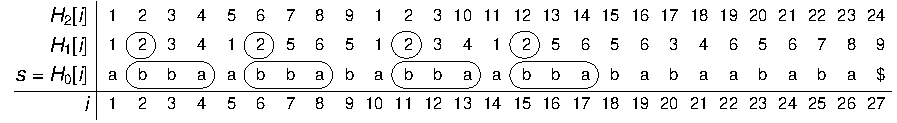
\includegraphics[width=0.98\textwidth,page=1]{fingerprint.pdf}
        \vspace{-.5cm}
    \end{center}
    \caption{\label{fig:fingerprint-ds}\fprintk\ data structure for $s=\textit{abbaabbababbaabbababaababa\$}$, $n=27$, $k=3$, $t_1=n^{1/3}=3$ and $t_2=n^{2/3}=9$. All substrings $\textit{bba}$ are highlighted with their $3$-length fingerprint $2$.}
\end{figure}



%%%%%%%%%%%%%%%%%%%%%%%%%%%%%%%%%%%%%%%%%%%%%%%%%%%%%%%%%%%%%%%%%%%%%%%%%%%%%%%
\subsection{Query\label{sec:fingerprint-query}}
The \fprintk\ query speeds up \proc{DirectComp} by comparing fingerprints of substrings of the input string instead of individual characters. The query algorithm consists of two traversals of the hierarchy of fingerprints. In the first traversal the algorithm compares progressively larger fingerprints of substrings until a mismatch is found and in the second traversal the algorithm compares progressively smaller substrings to find the precise point of the mismatch. The combination of these two traversals ensures both a fast worst case and average case performance. 

The details of the query algorithm are as follows. Given the \fprintk\ data structure, start with $v=0$ and $\ell=0$, then do the following steps:
\begin{samepage}
\begin{enumerate}
\item As long as $H_\ell[i+v] = H_\ell[j+v]$, increment $v$ by $t_\ell$, increment $\ell$ by one, and repeat this step unless $\ell = k-1$.
\item As long as $H_\ell[i+v] = H_\ell[j+v]$, increment $v$ by $t_\ell$ and repeat this step.
\item Stop and return $v$ when $\ell = 0$, otherwise decrement $\ell$ by one and go to step two.
\end{enumerate}

An example of a query is shown in \pref{fig:fingerprint-query}.
\end{samepage}

\begin{figure}[tb]
    \begin{center}
        \includegraphics[width=0.98\textwidth,page=2]{fingerprint.pdf}
        \vspace{-.5cm}
    \end{center}
    \caption{\label{fig:fingerprint-query}\fprintk\ query for $\LCE(3,12)$ on the data structure of \pref{fig:fingerprint-ds}. The top half shows how $H_\ell[i+v]$ moves through the data structure, and the bottom half shows $H_\ell[j+v]$.}
\end{figure}

\begin{lemma}\label{lem:query-correct}
The \fprintk\ query algorithm is correct.
\end{lemma}
\begin{proof}
At each step of the algorithm $v \leq \LCE(i,j)$, since the algorithm only increments $v$ by $t_\ell$ when it has found two matching fingerprints, and fingerprints of two substrings of the same length are only equal if the substrings themselves are equal. When the algorithm stops, it has found two fingerprints, which are not equal, and the length of these substrings is $t_\ell = 1$, therefore $v = \LCE(i,j)$.

The algorithm never reads $H_\ell[x]$, where $x>n$, because the string contains a unique character \$ at the end. This character will be at different positions in the substrings whose fingerprints are the last $t_\ell$ elements of $H_\ell$. These $t_\ell$ fingerprints will therefore be unique, and the algorithm will not continue at level $\ell$ after reading one of them.
\end{proof}

\begin{lemma}
The worst case query time for \fprintk\ is $O(k n^{1/k})$, and the average case query time is $O(1)$.
\end{lemma}
\begin{proof}
First we consider the worst case. Step one takes $O(k)$ time. In step two and three, the number of remaining characters left to check at level $\ell$ is $O(n^{(\ell+1)/k})$, since the previous level found two differing substrings of that length (at the top level $\ell=k-1$ we have $O(n^{(\ell+1)/k}) = O(n)$). Since we can check $t_\ell = \Theta(n^{\ell/k})$ characters in constant time at level $\ell$, the algorithm uses $O(n^{(\ell+1)/k})/\Theta(n^{\ell/k}) = O(n^{1/k})$ time at that level. Over all $k$ levels, $O(k n^{1/k})$ query time is used.

Next we consider the average case. At each step except step three, the algorithm increments $v$. Step three is executed the same number of times as step one, in which $v$ is incremented. The query time is therefore linear in the number of times $v$ is incremented, and it is thereby $O(v)$. From the proof of \pref{lem:query-correct} we have $v=\LCE(i,j)$. By Ilie et al.~\cite{ilie-navarro-tinta} the average $\LCE(i,j)$ is $O(1)$ and hence the average case query time is $O(1)$. 
\end{proof}

%%%%%%%%%%%%%%%%%%%%%%%%%%%%%%%%%%%%%%%%%%%%%%%%%%%%%%%%%%%%%%%%%%%%%%%%%%%%%%%
\paragraph{Average Case vs.\ Worst Case\label{sec:improved-avg}}
The first traversal in the query algorithm guarantees $O(1)$ average case performance. Without it the average case query time would be $O(k)$. However, the worst case bound would remain $O(kn^{1/k})$. Thus, for a better practical worst-case performance we could omit the first traversal entirely. We have extensively experimented with both variants and we found that in nearly all scenarios the first traversal improved the overall performance. In the cases where performance was not improved the first traversal only degraded the performance slightly. We therefore focus exclusively on the two traversal variant in the remainder of the paper. 


%query algorithm is optimized for average case. Without this, the average case query time would be $O(k)$, while the asymptotic worst case time would not be affected. The practical worst case query time could however be negatively affected. Our experiments have shown that the improvement in practical average case query time far outweighs any degraded worst case performance, and for small values of $k$, changes in worst case performance are barely measurable.

%Our experiments have shown that for small values of $k$, optimizing for the average case significantly improves average case query time, while any negative effect on worst case query time is barely measurable. For large values of $k$ the improvement in average case far outweighs the slightly degraded practical worst case.

\begin{comment}
We could have left out step one of the query algorithm and started with $\ell=k-1$. This would keep the asymptotic worst case query time of $O(k n^{1/k})$, while it might improve practical worst case query time, but it would increase our average case query time to $O(k)$.
Our experiments have shown that whenever $k$ is small, keeping step one improves average case query time, while it does not have a measurable effect on worst case query times. When $k = \logceil$, keeping step one can double the worst case query time, while it can make the average case query time 40 times faster for an input string of ten million characters. We want to optimize our LCE query time for the average case where the LCE value is small, so our results in \pref{sec:results} does not include the variant of \fprintk\ with $O(k)$ average case query time.

%\begin{figure}[tp]
%    \begin{center}
%        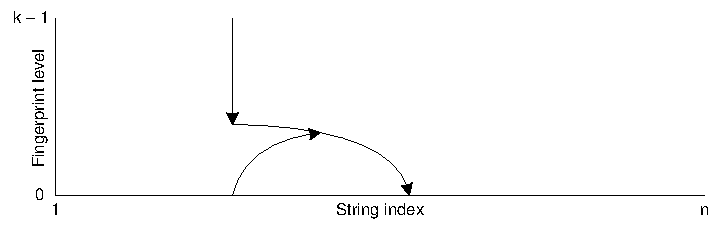
\includegraphics[width=1\textwidth,page=1]{fingerprint-updown.pdf}
%    \end{center}
%    \caption{\label{fig:fingerprint-updown}Two ways of querying the fingerprint levels, one starting from level $\ell=k-1$ and one starting at level $\ell=0$.}
%\end{figure}

In step one of our query algorithm we perform one comparison at each level. We could instead do up to $O(n^{1/k})$ comparisons at each level without affecting asymptotic times.
Our experiments have shown that always doing one comparison at each level is the best in practice.
\end{comment}

%%%%%%%%%%%%%%%%%%%%%%%%%%%%%%%%%%%%%%%%%%%%%%%%%%%%%%%%%%%%%%%%%%%%%%%%%%%%%%%
\subsection{Preprocessing}

The tables of fingerprints use $O(k n)$ space. In the case with $k=\logceil$ levels, the data structure is the one generated by Karp-Miller-Rosenberg~\cite{karp-miller-rosenberg}. This data structure can be constructed in $O(n\log n)$ time. With $k<\logceil$ levels, KMR can be adapted, but it still uses $O(n\log n)$ preprocessing time.

We can preprocess the data structure in $O(\sortt + k n)$ time using the SA and LCP arrays. First create the SA and LCP arrays. Then preprocess each of the $k$ levels using the following steps:
\begin{samepage}
\begin{enumerate}
\item Loop through the $n$ substrings of length $t_\ell$ in lexicographically sorted order by looping through the elements of SA.
\item Assign an arbitrary fingerprint to the first substring.
\item If the current substring $s[\SA[i]\twodots\SA[i]+t_\ell-1]$ is equal to the substring examined in the previous iteration of the loop, give the current substring the same fingerprint as the previous substring, otherwise give the current substring a new unused fingerprint. The two substrings are equal when $\LCE[i] \geq t_\ell$.
\end{enumerate}

An example is shown in \pref{fig:fingerprint-preproc}.
\end{samepage}

\begin{figure}[tb]
    \begin{center}
        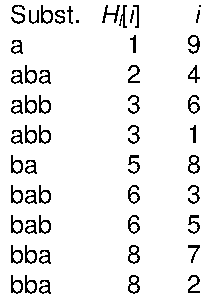
\includegraphics[width=0.2\textwidth,page=1]{fingerprint-preproc.pdf}
        \vspace{-.5cm}
    \end{center}
    \caption{\label{fig:fingerprint-preproc}The first column lists all substrings of $s=abbababba$ with length $t_\ell = 3$. The second column lists fingerprints assigned to each substring. The third column lists the position of each substring in $s$.}
\end{figure}

\begin{lemma}
The preprocessing algorithm described above generates the data structure described in \pref{sec:fingerprint-ds}.
\end{lemma}

\begin{proof}
We always assign two different fingerprints whenever two substrings are different, because whenever we see two differing substrings, we change the fingerprint to a value not previously assigned to any substring.

We always assign the same fingerprint whenever two substrings are equal, because all substrings, which are equal, are grouped next to each other, when we loop through them in lexicographical order.
\end{proof}

\begin{samepage}
\begin{lemma}
The preprocessing algorithm described above takes $O(\sortt + k n)$ time.
\end{lemma}
\begin{proof}
We first construct the SA and LCP arrays, which takes $O(\sortt)$ time~\cite{sort-complexity}. We then preprocess each of the $k$ levels in $O(n)$ time, since we loop through $n$ substrings, and comparing neighboring substrings takes constant time when we use the LCP array. The total preprocessing time becomes $O(\sortt\\ + k n)$.
\end{proof}
\end{samepage}

%%%%%%%%%%%%%%%%%%%%%%%%%%%%%%%%%%%%%%%%%%%%%%%%%%%%%%%%%%%%%%%%%%%%%%%%%%%%%%%
%%%%%%%%%%%%%%%%%%%%%%%%%%%%%%%%%%%%%%%%%%%%%%%%%%%%%%%%%%%%%%%%%%%%%%%%%%%%%%%
\section{Experimental Results\label{sec:results}}

In this section we show results of actual performance measurements. The measurements were done on a Windows 23-bit machine with an Intel P8600 CPU (3 MB L2, 2.4 GHz) and 4 GB RAM. The code was compiled using GCC 4.5.0 with \texttt{-O3}.

%%%%%%%%%%%%%%%%%%%%%%%%%%%%%%%%%%%%%%%%%%%%%%%%%%%%%%%%%%%%%%%%%%%%%%%%%%%%%%%
\subsection{Tested Algorithms}

We implemented different variants of the \fprintk\ algorithm in C++ and compared them with optimized versions of the \proc{DirectComp} and \proc{LcpRmq} algorithms. The algorithms we compared are the following:
\begin{description}
\item[\proc{DirectComp}] is the simple \proc{DirectComp} algorithm with no preprocessing and worst case $O(n)$ query time.
\item[\fprintk\textless$t_{k-1}$, ..., $t_1$\textgreater ac] is the \fprintk\ algorithm using $k$ levels, where $k$ is $2$, $3$ and $\logceil$. The numbers \textless$t_{k-1}$, ..., $t_1$\textgreater\ describe the exact size of fingerprinted substrings at each level.
\item[\proc{RMQ}\textless$n$, $1$\textgreater] is the \proc{LcpRmq} algorithm using constant time RMQ.
\end{description}

%%%%%%%%%%%%%%%%%%%%%%%%%%%%%%%%%%%%%%%%%%%%%%%%%%%%%%%%%%%%%%%%%%%%%%%%%%%%%%%
\subsection{Test Inputs and Setup}

We have tested the algorithms on different kinds of strings:
\begin{description}
\item[Average case strings] These strings have many small LCE values, such that the average LCE value over all $n^2$ query pairs is less than one. We use results on these strings as an indication average case query times over all input pairs $(i,j)$ in cases where most or all LCE values are small on expected input strings. We construct these strings by choosing each character uniformly at random from an alphabet of size 10
\item[Worst case strings] These strings have many large LCE values, such that the average LCE value over all $n^2$ query pairs is $n/2$. We use results on these strings as an indication of worst case query times, since the query times for all tested algorithms are asymptotically at their worst when the LCE value is large. We construct these strings with an alphabet size of one.
\item[Medium LCE value strings] These strings have an average LCE value over all $n^2$ query pairs of $n/2r$, where $r=0.73n^{0.42}$. These strings where designed to show that \fprint\ can be faster than both \proc{DirectComp} and \proc{LcpRmq} on some inputs between the average case and worst case. The strings consist of repeating substrings of $r$ unique characters.
%The value of $r$ is a power regression over $(r,n) = (5,100)$, $(15,1.000)$, $(35,10.000)$ and $(100,100.000)$, where each of the values of $n$ were chosen such that \fprintk\ was faster than both \proc{DirectComp} and \proc{LcpRmq} on a plot with the given constant value of $r$. 
\end{description}

Each measurement we make is an average of query times over a million random query pairs $(i, j)$. For a given string length and string type (worst case strings vs.\ average case strings), we use the same string and the same million query pairs on all tested algorithms.

\begin{comment}
For each kind of strings, we tested the algorithms using the following pattern:
\begin{enumerate}
\item Generate a string of length $n$ and generate a million random pairs $(i, j)$, where each of $i$ and $j$ is chosen between $1$ and $n$ uniformly at random.
\item For each tested algorithm, preprocess the given string, and run a query for each of the million pairs. Measure the time it takes to run all the queries combined.
\item Double the value of $n$ and repeat from step one.
\end{enumerate}
\end{comment}

\subsection{Results}

\begin{figure}[tb]
    \begin{center}
        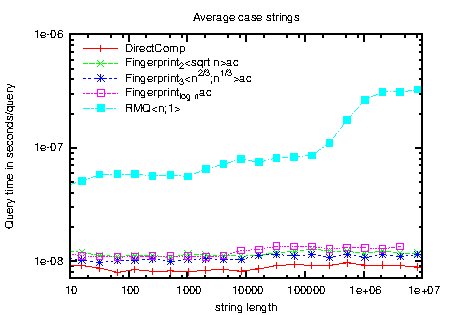
\includegraphics[width=0.49\textwidth,type=pdf,ext=.pdf,read=.pdf]{length-article-rand10.plt}
        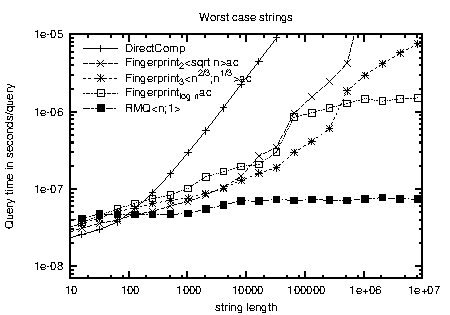
\includegraphics[width=0.49\textwidth,type=pdf,ext=.pdf,read=.pdf]{length-article-alla.plt}
        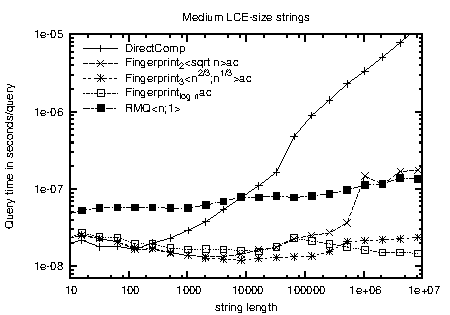
\includegraphics[width=0.49\textwidth,type=pdf,ext=.pdf,read=.pdf]{length-article-repeat-pow.plt}
    \end{center}
    \caption{\label{fig:test-fingerprint}Comparison of our new \fprintk\ algorithm for $k=2$, $k=3$ and $k=\logceil$ versus the existing \proc{DirectComp} and \proc{LcpRmq} algorithms.}
\end{figure}

\begin{table}[tb]
\centering
\begin{tabular}{l|r|r|r|r|r|r|r}
\hline\hline
% File & \proc{DirectComp} & \fprint[2]\textless$\sqrt n$\textgreater ac & \fprint[3]\textless$n^{2/3}$, $n^{1/3}$\textgreater ac & \fprint[\log n]ac & RMQ<n;1> \\ [0.5ex] \hline
File & $n$ & $\sigma$ & DC & FP$_2$ & FP$_3$ & FP$_{\log n}$ & RMQ \\ [0.5ex] \hline
book1 & $0.7\cdot 2^{20}$ & 82 & 8.1 & 11.4 & 10.6 & 12.0 & 218.0 \\ \hline
kennedy.xls & $1.0\cdot 2^{20}$ & 256 & 11.9 & 16.0 & 16.1 & 18.6 & 114.4 \\ \hline
E.coli & $4.4\cdot 2^{20}$& 4 & 12.7 & 16.5 & 16.6 & 19.2 & 320.0 \\ \hline
bible.txt & $3.9\cdot 2^{20}$ & 63 & 8.5 & 11.3 & 10.5 & 12.6 & 284.0 \\ \hline
world192.txt & $2.3\cdot 2^{20}$ & 93 & 7.9 & 10.5 & 9.8 & 12.7 & 291.7 \\ \hline \\
\end{tabular}
\caption{Query times in nano seconds for \proc{DirectComp} (DC), \fprintk\ (FP$_k$) and \proc{LcpRmq} (RMQ) on the five largest files from the Canterbury corpus.}\label{tab:text-fprint-files}
\end{table}

\pref{fig:test-fingerprint} shows our experimental results on average case strings with a small average LCE value, worst case strings with a large average LCE value, and strings with a medium average LCE value.

On average case strings, our new \fprintk\ algorithm is approximately 20\% slower than \proc{DirectComp}, and it is between than 5 and 25 times faster than \proc{LcpRmq}. We see the same results on some real world strings in \pref{tab:text-fprint-files}.

On worst case strings, the \fprintk\ algorithms are significantly better than \proc{DirectComp} and somewhat worse than \proc{LcpRmq}. Up until $n=30.000$ the three measured \fprintk\ algorithms have nearly the same query times. Of the \fprintk\ algorithms, the $k=2$ variant has a slight advantage for small strings of length less than around $2.000$. For longer strings the $k=3$ variant performs the best up to strings of length $250.000$, at which point the $k=\logceil$ variant becomes the best. This indicates that for shorter strings, using fewer levels is better, and when the input size increases, the \fprintk\ variants with better asymptotic query times have better worst case times in practice.

On the plot of strings with medium average LCE values, we see a case where our \fprintk\ algorithms are faster than both \proc{DirectComp} and \proc{LcpRmq}.

We conclude that our new \fprintk\ algorithm achieves a tradeoff between worst case times and average case times, which is better than the existing best \proc{DirectComp} and \proc{LcpRmq} algorithms, yet it is not strictly better than the existing algorithms on all inputs. \fprintk\ is therefore a good choice in cases where both average case and worst case performance is important.

%  \fprint[3]\ also shows such a jump, but for greater input sizes, as it uses less memory.

\proc{LcpRmq} shows a significant jump in query times around $n=1.000.000$ on the plot with average case strings, but not on the plot with worst case strings. We have run the tests in Cachegrind, and found that the number of instructions executed and the number of data reads and writes are exactly the same for both average case strings and worst case strings. The cache miss rate for average case strings is 14\% and 9\% for the L1 and L2 caches, and for worst case strings the miss rate is 17\% and 13\%, which is the opposite of what could explain the jump we see in the plot.

% \fixme{Results: Investigate if we can explain the jump in Fingerprint-log}
% \paragraph{\fprint[\log n] cache limit.}
% \proc{LcpRmq} uses more space than all of \proc{DirectComp}, \fprint[2] and \fprint[3], so it is expected that it reaches the cache limit before these. However \fprint[\log n] uses more space than \proc{LcpRmq} at the input sizes we measure, since \proc{LcpRmq} uses the same amount of memory as \fprint[6], and $\lceil\log(10.000.000)\rceil = 24$. However, the \fprintk\ algorithms only access the lowest levels of their data structure whenever the LCE values are small, and there is therefore no visible jump due to cache limits for \fprint[\log n] on the plot with average case strings. On the plot with worst case strings however, we see a jump in \fprint[\log n] between $n=20.000$ and $n=50.000$, since it uses all its $\logceil$ levels when the LCE values are large.

%%%%%%%%%%%%%%%%%%%%%%%%%%%%%%%%%%%%%%%%%%%%%%%%%%%%%%%%%%%%%%%%%%%%%%%%%%%%%%%
\subsection{Cache Optimization}

\begin{figure}[tb]
    \begin{center}
        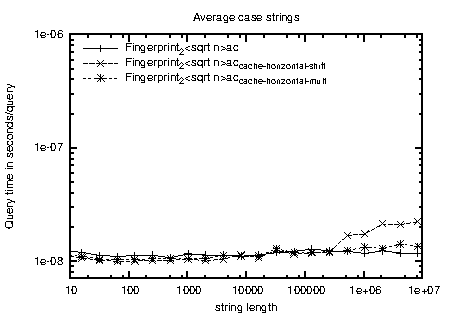
\includegraphics[width=0.49\textwidth,type=pdf,ext=.pdf,read=.pdf]{length-fingerprint-cache-rand10.plt}
        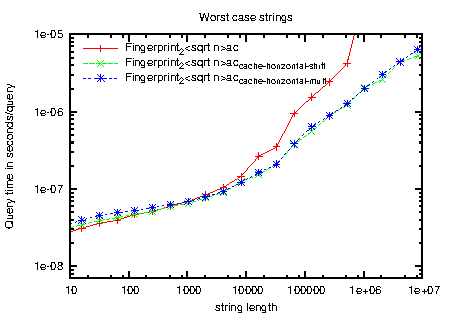
\includegraphics[width=0.49\textwidth,type=pdf,ext=.pdf,read=.pdf]{length-fingerprint-cache-alla.plt}
        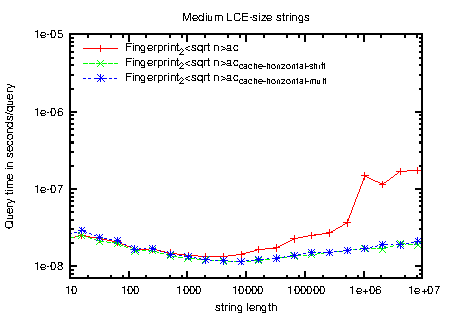
\includegraphics[width=0.49\textwidth,type=pdf,ext=.pdf,read=.pdf]{length-fingerprint-cache-repeat-pow.plt}
        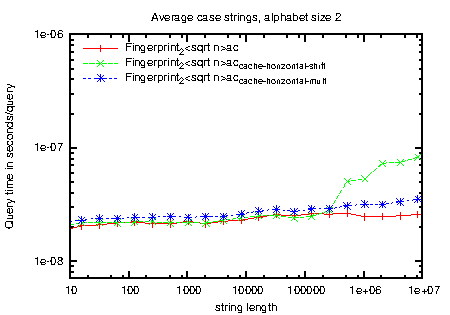
\includegraphics[width=0.49\textwidth,type=pdf,ext=.pdf,read=.pdf]{length-fingerprint-cache-rand2.plt}
    \end{center}
    \caption{\label{fig:plot-fingerprint-cache-horiz}Query times of \fprint[2] with and without cache optimization.}
\end{figure}

\begin{figure}[tb]
    \begin{center}
        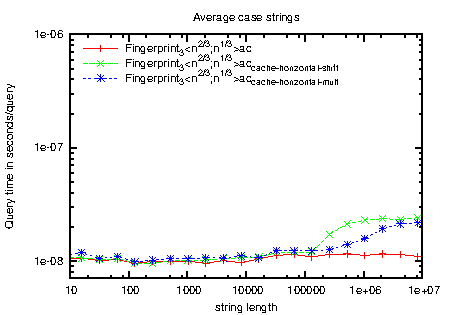
\includegraphics[width=0.49\textwidth,type=pdf,ext=.pdf,read=.pdf]{length-fingerprint3-cache-rand10.plt}
        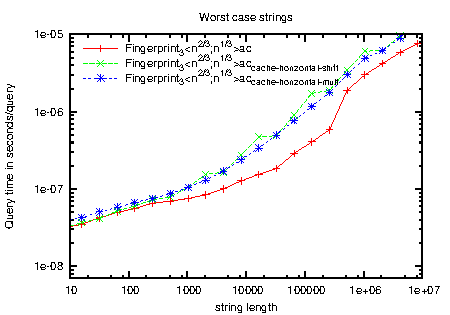
\includegraphics[width=0.49\textwidth,type=pdf,ext=.pdf,read=.pdf]{length-fingerprint3-cache-alla.plt}
        \vspace{-.5cm}
    \end{center}
    \caption{\label{fig:plot-fingerprint3-cache}Query times of \fprint[3] with and without cache optimization.}
\end{figure}

%\paragraph{Horizontal, intra-level optimization}

The amount of I/O used by \fprintk\ is $O(k n^{1/k})$. However if we structure our tables of fingerprints differently, we can improve the number of I/O operations to $O(k(n^{1/k}/B+1))$ in the cache-oblivious model. Instead of storing $F_{t_\ell}[i]$ at $H_\ell[i]$, we can store it at $H_\ell[((i-1)\mod t_\ell)\cdot\lceil n/t_\ell\rceil+\lfloor (i-1)/t_\ell\rfloor+1]$. This will group all used fingerprints at level $\ell$ next to each other in memory, such that the amount of I/O at each level is reduced from $O(n^{1/k})$ to $O(n^{1/k}/B)$.

The size of each fingerprint table will grow from $|H_\ell| = n$ to $|H_\ell| = n+t_\ell$, because the rounding operations may introduce one-element gaps in the table after every $n/t_\ell$ elements. We achieve the greatest I/O improvement when $k$ is small. When $k=\logceil$, this cache optimization gives no asymptotic difference in the amount of I/O.

We have implemented two cache optimized variants. One as described above, and one where multiplication, division and modulo is replaced with shift operations. To use shift operations, $t_\ell$ and $\lceil n/t_\ell\rceil$ must both be powers of two. This may double the size of the used address space.

\pref{fig:plot-fingerprint-cache-horiz} shows our measurements for \fprint[2]. On average case strings the cache optimization does not change the query times, while on worst case strings and strings with medium size LCE values, cache optimization gives a noticeable improvement for large inputs. The cache optimized \fprint[2] variant with shift operations shows an increase in query times for large inputs, which we cannot explain.
%
The last plot on \pref{fig:plot-fingerprint-cache-horiz} shows a variant of average case where the alphabet size is changed to two. This plot shows a bad case for cache optimized \fprint[2]. LCE values in this plot are large enough to ensure that $H_1$ is used often, which should make the extra complexity of calculating indexes into $H_1$ visible. At the same time the LCE values are small enough to ensure, that the cache optimization has no effect. In this bad case plot we see that the cache optimized variant of \fprint[2] has only slightly worse query time compared to the variant, which is not cache optimized. \pref{fig:plot-fingerprint3-cache} shows the measurements for \fprint[3]. Unlike \fprint[2], the cache optimized variant is slightly slower than the unoptimized variant. Hence, our cache optimization is effective for $k=2$ but not $k=3$. 


%%%%%%%%%%%%%%%%%%%%%%%%%%%%%%%%%%%%%%%%%%%%%%%%%%%%%%%%%%%%%%%%%%%%%%%%%%%%%%%
\section{Conclusions}

We have presented the \fprintk\ algorithm, where $k$ is a parameter $1 \leq k \leq \logceil$, which for a string $s$ of length $n$ and alphabet size $\sigma$, can solve the LCE problem in $O(k n^{1/k})$ worst case query time and $O(1)$ average case query time using $O(k n)$ space and $O(\sortt + k n)$ preprocessing time.

The \fprintk\ algorithm is able to achieve a balance between practical worst case and average case query times. It has almost as good average case query times as \proc{DirectComp}, its worst case query times are significantly better than those of \proc{DirectComp}, and we have shown cases between average and worst case where \fprintk\ is better than both \proc{DirectComp} and \proc{LcpRmq}. \fprintk\ gives a good time space tradeoff, and it uses less space than \proc{LcpRmq} when $k$ is small. %The performance of \fprintk\ can be tweaked on many parameters, and we have found that optimizing for average case queries and for memory caches improve practical query time performance.

%%%%%%%%%%%%%%%%%%%%%%%%%%%%%%%%%%%%%%%%%%%%%%%%%%%%%%%%%%%%%%%%%%%%%%%%%%%%%%%
%%%%%%%%%%%%%%%%%%%%%%%%%%%%%%%%%%%%%%%%%%%%%%%%%%%%%%%%%%%%%%%%%%%%%%%%%%%%%%%
\begin{thebibliography}{9}
\bibitem{sort-complexity} M. Farach-Colton, P. Ferragina, and S. Muthukrishnan. On the sorting-complexity of suffix tree construction. \textit{J. ACM} 47(6):987-1011, 2000.

\bibitem{jf-rmq} J. Fischer, and V. Heun. Theoretical and Practical Improvements on the RMQ-Problem, with Applications to LCA and LCE. In \textit{Proc. 17th CPM}, pages 36-48, 2006.

\bibitem{nca} D. Harel, R. E. Tarjan. Fast Algorithms for Finding Nearest Common Ancestors. \textit{SIAM J. Comput.}, 13(2):338-355, 1984.

\bibitem{ilie-navarro-tinta} L. Ilie, G. Navarro, and L. Tinta. The longest common extension problem revisited and applications to approximate string searching. \textit{J. Disc. Alg.,} 8(4):418-428, 2010.

\bibitem{karp-miller-rosenberg} R. M. Karp, R. E. Miller, and A. L. Rosenberg. Rapid identification of repeated patterns in strings, trees and arrays. In \textit{Proc. 4th STOC}, pages 125-136, 1972.

\bibitem{approx-search} Gad M. Landau and Uzi Vishkin. Introducing efficient parallelism into approximate string matching and a new serial algorithm. In \textit{Proc. 18th STOC}, pages 220-230, 1986.

\end{thebibliography}

%\fxfatal{Opskriv funktioner for plads.}

\end{document}
